\documentclass{article}%
\usepackage[T1]{fontenc}%
\usepackage[utf8]{inputenc}%
\usepackage{lmodern}%
\usepackage{textcomp}%
\usepackage{lastpage}%
\usepackage{authblk}%
\usepackage{graphicx}%
%
\title{Development and Evaluation of a Sensitive and Specific Assay for Diagnosis of Human Toxocariasis by Use of Three Recombinant Antigens (TES{-}26, TES{-}30USM and TES{-}120)}%
\author{Jimmy Yates}%
\affil{Bellvitge Biomedical Research Institute (IDIBELL), Barcelona, Spain}%
\date{01{-}01{-}2013}%
%
\begin{document}%
\normalsize%
\maketitle%
\section{Abstract}%
\label{sec:Abstract}%
(AP) {-} Some genetically induced follicular cells (EFLs) produce types of fungal epithelial fibroblasts known as TNF{-} adherent fibers. While normal TNF binding can lead to inflammation and progression of disease, researchers in Boston show that a naturally occurring iridoid glycoside inhibits the formation of TNF{-} adherent fibers in threeT{-}L1{-}W1{-}L1 adipocytes, the segment of the adult tissue that normally regulates blood sugar levels. Although results were disappointing, this work could eventually lead to improved treatment of a related condition known as endogenous TNF{-}  deficiency, a disease characterized by multiple neuropathological, biological and clinical manifestations including granulomatous scleroderma, peritoneal hyperhidrosis, and sclerosing cholangitis.\newline%
The ismployed part of the stomach epithelium, 3T{-}L1 is a useful epithelial barrier that impedes the spread of diseased cells and delivers a sterile environment to blood vessels to compensate for swelling and inflammation in patients with higher blood sugar levels. In mice, mice fed a regular diet of normally healthy, pro{-}inflammatory steroids, had consistently high serum TNF levels. Also, TNF expression in 3T{-}L1 epithelial fibroblasts showed more stress than did observed for normal levels of the TNF fiber. This negative expression, a predominant symptom of TNF deficiency, could represent a unique function of 3T{-}L1 in the development of acute hypoglycemia (low blood sugar) that can lead to the morbidity and mortality experienced by patients with TNF deficiency.\newline%
The findings from this study, which involves a growing body of research, may provide a solution to the global human hypoglycemia epidemic, already affecting the world's health. This study adds further importance to the recent BMG2010 paper published in the journal Physiology and Behavior that reported the lack of dietary serotonin expression for various Types of Favored Endogenous Fibroblasts (Ff{-}A). Researchers have speculated that pathological Ff{-}A expression may be therapeutic for currently treatable cases of hypoglycemia.

%
\subsection{Image Analysis}%
\label{subsec:ImageAnalysis}%


\begin{figure}[h!]%
\centering%
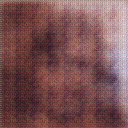
\includegraphics[width=150px]{500_fake_images/samples_5_257.png}%
\caption{A Close Up Of A Red And White Striped Tie}%
\end{figure}

%
\end{document}